\chapter{Implementations} \label{ch:implementations}
\vcomment{This chapter shows how things described within the research protocol are performed. By separating it out, I can focus on things like verifying accuracy / comparisons / demos / pseudocode without cluttering up the discussion of the actual methodologies of the next chapter. That way parameters choices, etc. can be more clearly highlighted. However, this section is apt place to discuss how varying parameters influences whatever methods are being used.}


\section{Calculating the Hessian via FFT}

% assuming that we already know how the 
Efficient implementation of the Frangi filter ultimately relies on performing Gaussian blur in frequency space. Here we demonstrate that our FFT implementation of Gaussian blur is commensurate with other implementations. 

In \cref{fig:fft-gaussian-demo}, we demonstrate the compatibility of standard convolution and FFT convolve. Each row corresponds to a different scale at which Gaussian blurring  occurs. Column (a) is standard convolution with a sampled Gaussian kernel, column (b) is FFT-convolution with a Gaussian kernel, and column (c) is a FFT-convolution with the ``discrete Gaussian kernel''. In column (d), the 1D discrete Gaussian kernel (in green) is plotted against the sampled continuous Gaussian kernel (in black). Note that each of the images in the first three columns are scaled the same.
\begin{figure}
  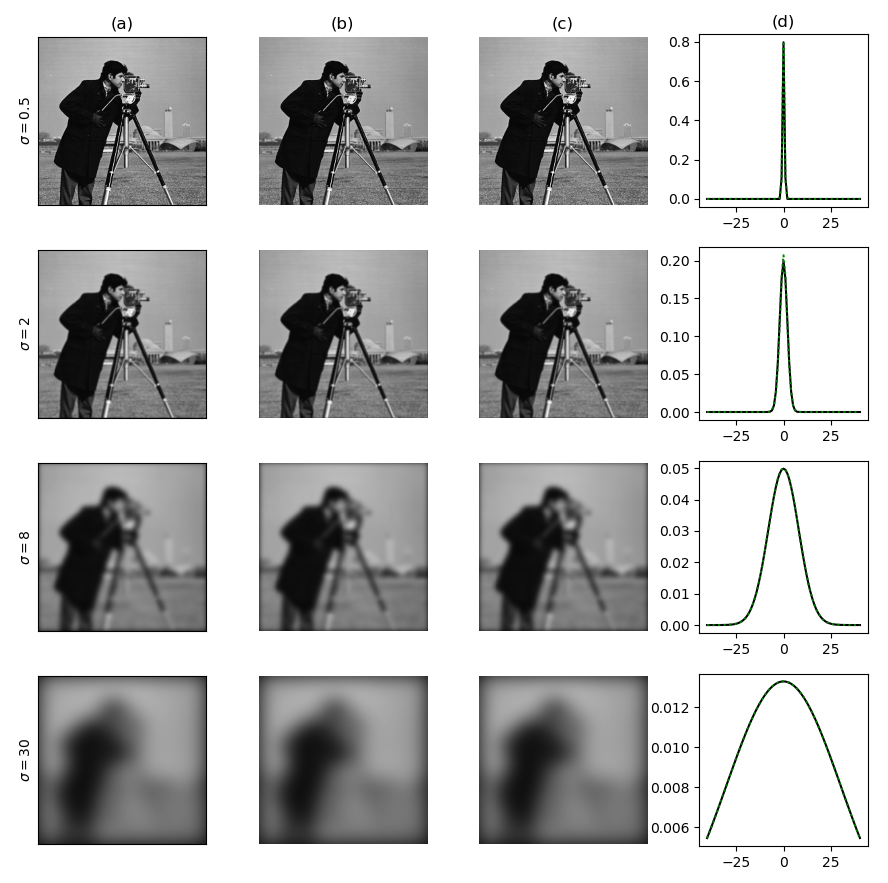
\includegraphics[width=\linewidth]{fft_gaussian_demo}
  \caption{Compatibility of Gaussian convolution strategies}
  \label{fig:fft-gaussian-demo}
\end{figure}

In \cref{fig:semigroup-demo}, we show these same three methods of Gaussian blur but for a large scale
($\sigma=45$). For each method of taking the Gaussian blur ((a) - standard convolution with sampled kernel, (b) fft with sampled kernel, (c) fft with discrete kernel), the top row is one round of Gaussian blur with $\sigma=45$ and the bottom row is two progressive passes of Gaussian blur ($\sigma_1 = 10, \sigma_2 = 35$). The mean squared error and mean absolute error between the one-pass and two-pass versions are outputted below. Code for this demo can be found in \texttt{hfft.semigroup\_demo}.
The discrete kernel performs very slightly better than the sampled versions. We originally attempted
this demonstration with a much larger sigma (say $\sigma=150$) and multiple iterations, but unfortunately multiple passes cause the ``noise'' from zeroing out around the boundaries to become very noticable after several iterations (here, we've opted to crop out a radius of pixels from around the edges equal to the standard deviation of the Gaussian before we calculated the MAE or MSE). We could show this again with a zero border or maybe even just a 1D signal.

\begin{table}
  \centering
  \begin{tabular}{c|cc}
   blurring method   & MSE & MAE \\
    \hline
spatial convolution, sampled kernel & 0.00054426 & 0.02015643 \\
FFT convolution, sampled kernel & 0.00055205 & 0.02029916 \\
FFT convolution, discrete kernel & 0.00054406 & 0.02015336
    \end{tabular}
\end{table}


\begin{figure}
  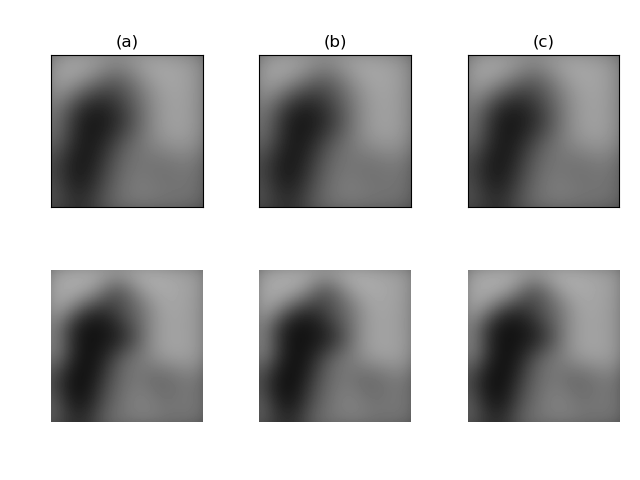
\includegraphics[width=\linewidth]{semigroup_demo}
  \caption{Iterative Gaussian blur}
  \label{fig:semigroup-demo}
\end{figure}

We further confirm the commensurate nature of Gaussian blur techniques by comparing the three techniques on a placental image and using each to calculate Frangi targets. The code can be found in \texttt{hfft\_accuracy.py}. In \cref{tab:mse-G-sigma-0.3}, \cref{tab:mse-F-sigma-0.3}, \cref{tab:mse-G-sigma-5} and \cref{tab:mse-F-sigma-5} we compare the mean squared error of a single image blurred (A) with standard spatial convolution, (B) with FFT sampled Gaussian kernel, and (C) with the discrete kernel. We see that the standard convolution and discrete convolution are very similar, while the sampled discrete Gaussian is off by two orders of magnitude, but still reasonably small. We further confirm these by viewing the intensity of the images and the Frangi targets themselves across an arbitrarily chosen horizontal cross section of the image. As seen in \cref{fig:cross-sec-G-sigma=0.3}, \cref{fig:cross-sec-F-sigma=0.3},
\cref{fig:cross-sec-G-sigma=5}, \cref{fig:cross-sec-F-sigma=5}, the peaks of the Gaussian blurred image all still occur at the same places, as do the Frangi responses. We repeated this procedure up to $\sigma=90$ and found a situation similar to $\sigma=5$; it was only in very small scales where there was any noticeable difference at all.




******************************************************************************** 


\begin{table}
  \parbox{.45\linewidth}{
  \centering
  \begin{tabular}{c|ccc}
    &  A & B & C \\
    \hline
  A & -  & 1.296e-03 & 6.772e-06 \\
  B & -  & - & 1.247e-03 \\
  C & -  &  - &  - \\
  \end{tabular}
\caption{MSE of Gaussian blurs of an image ($\sigma=0.3$)}
\label{tab:mse-G-sigma-0.3}
}
    \parbox{.45\linewidth}{
  \centering
  \begin{tabular}{c|ccc}
      &  A &  B         & C \\
      \hline
    A &  - &  4.256e-06 & 5.537e-08 \\
    B &  - &  -         & 4.337e-06 \\
    C &  - &  -         &  - \\
  \end{tabular}
  \caption{MSE of Frangi scores $\sigma=0.3$}
  \label{tab:mse-F-sigma-0.3}
}
  \end{table}



\begin{figure}
  \centering
  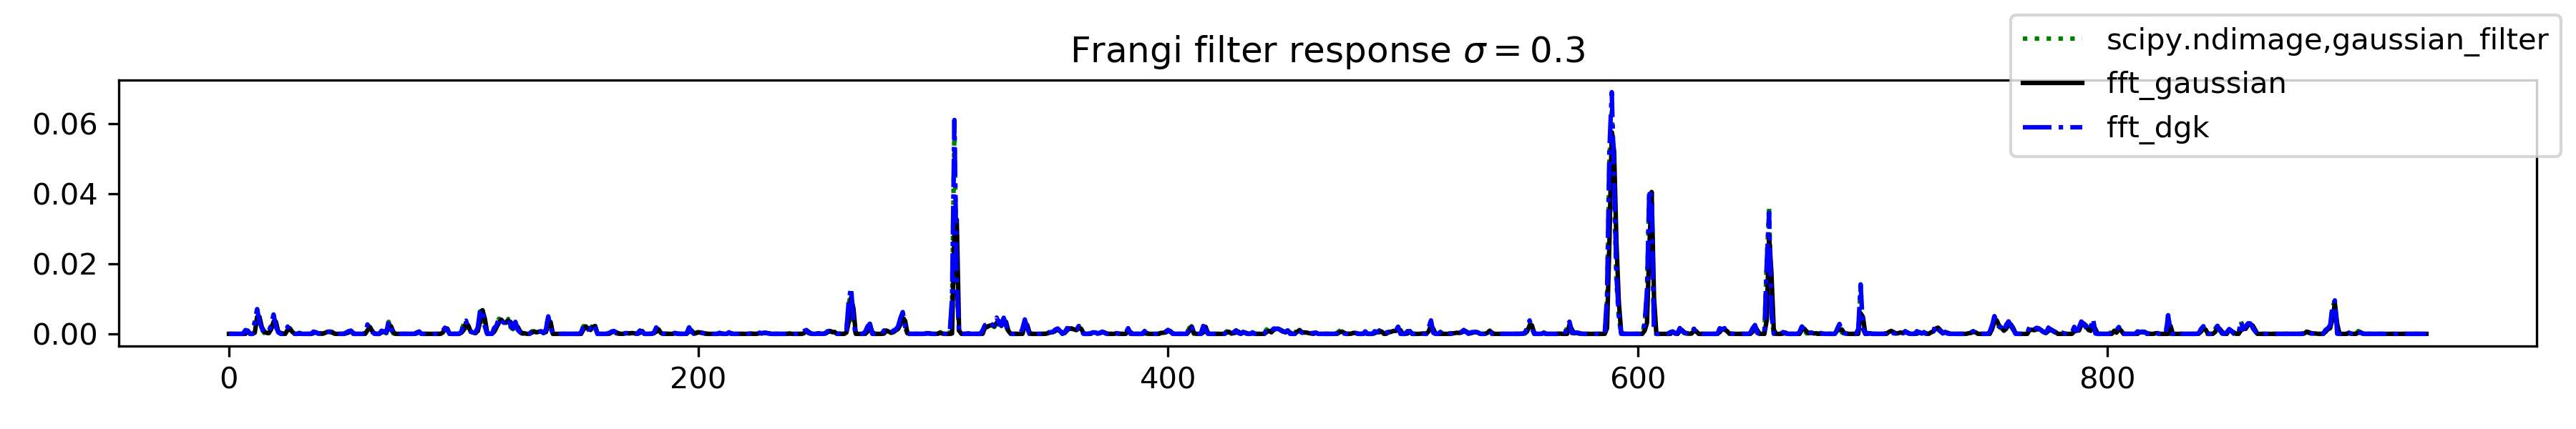
\includegraphics[width=\linewidth]{Fslice_sigma=3}
  \caption{Image cross-section of Gaussian blurred images}
  \label{fig:cross-sec-G-sigma=0.3}
\end{figure}

\begin{figure}
  \centering
  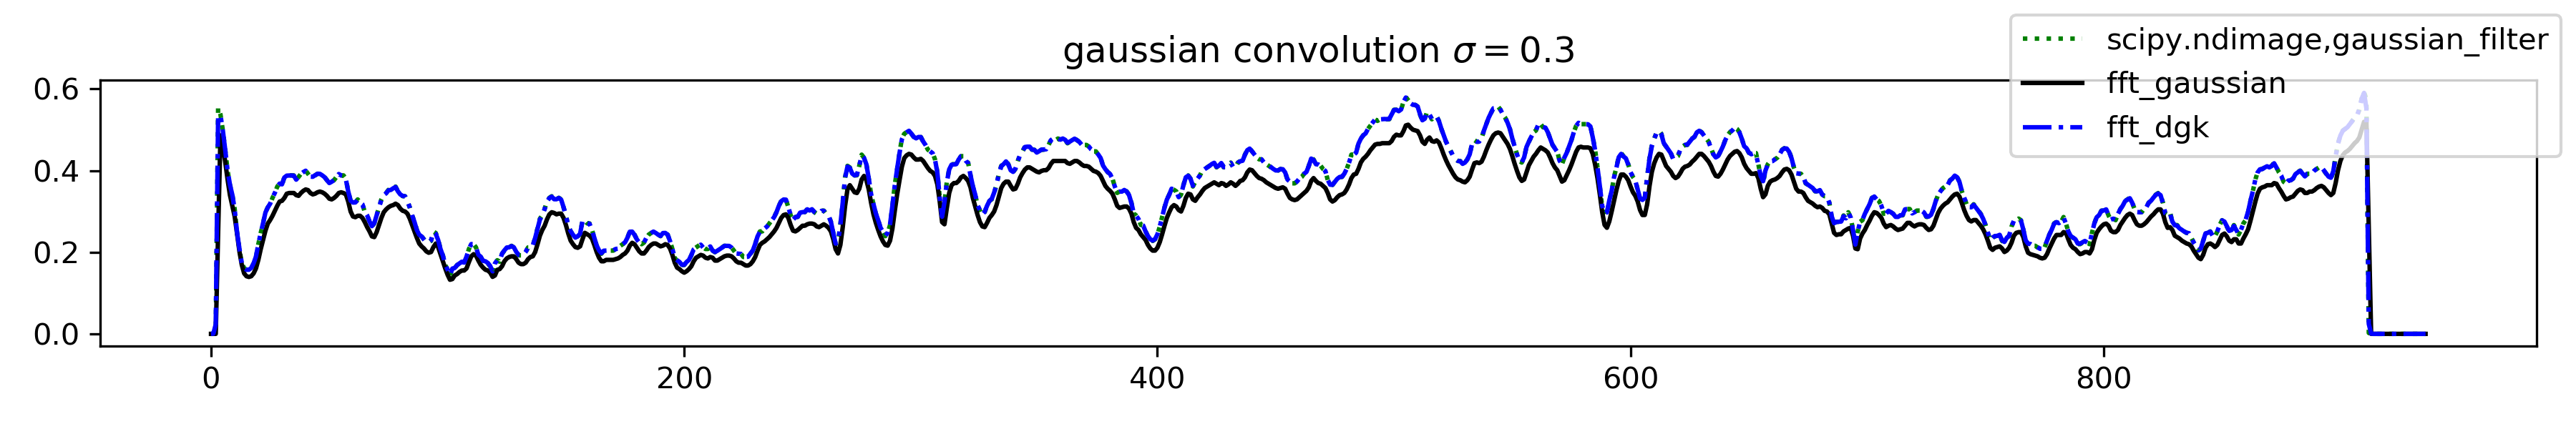
\includegraphics[width=\linewidth]{Gslice_sigma=3}
    \caption{Image cross-section of Frangi targets images}
    \label{fig:cross-sec-F-sigma=0.3}
\end{figure}



\begin{table}
  \parbox{.45\linewidth}{
    \centering
    \begin{tabular}{c|ccc}
      &  A & B & C \\
      \hline
      A & -  &  9.012e-06 & 8.629e-09 \\
      B & -  & - & 9.031e-06 \\
      C & -  &  - &  - \\
    \end{tabular}
    \caption{MSE of Gaussian blurs of an image ($\sigma=5$)}
    \label{tab:mse-G-sigma-5}
  }
  \parbox{.45\linewidth}{
    \centering
    \begin{tabular}{c|ccc}
      &  A &  B         & C \\
      \hline
      A &  - &  9.388e-05 8.383e-07 \\
      B &  - &  -         & 9.599e-05 \\
      C &  - &  -         &  - \\
    \end{tabular}
    \caption{MSE of Frangi scores $\sigma=5$}
    \label{tab:mse-F-sigma-5}
  }
\end{table}

\begin{figure}
  \centering
  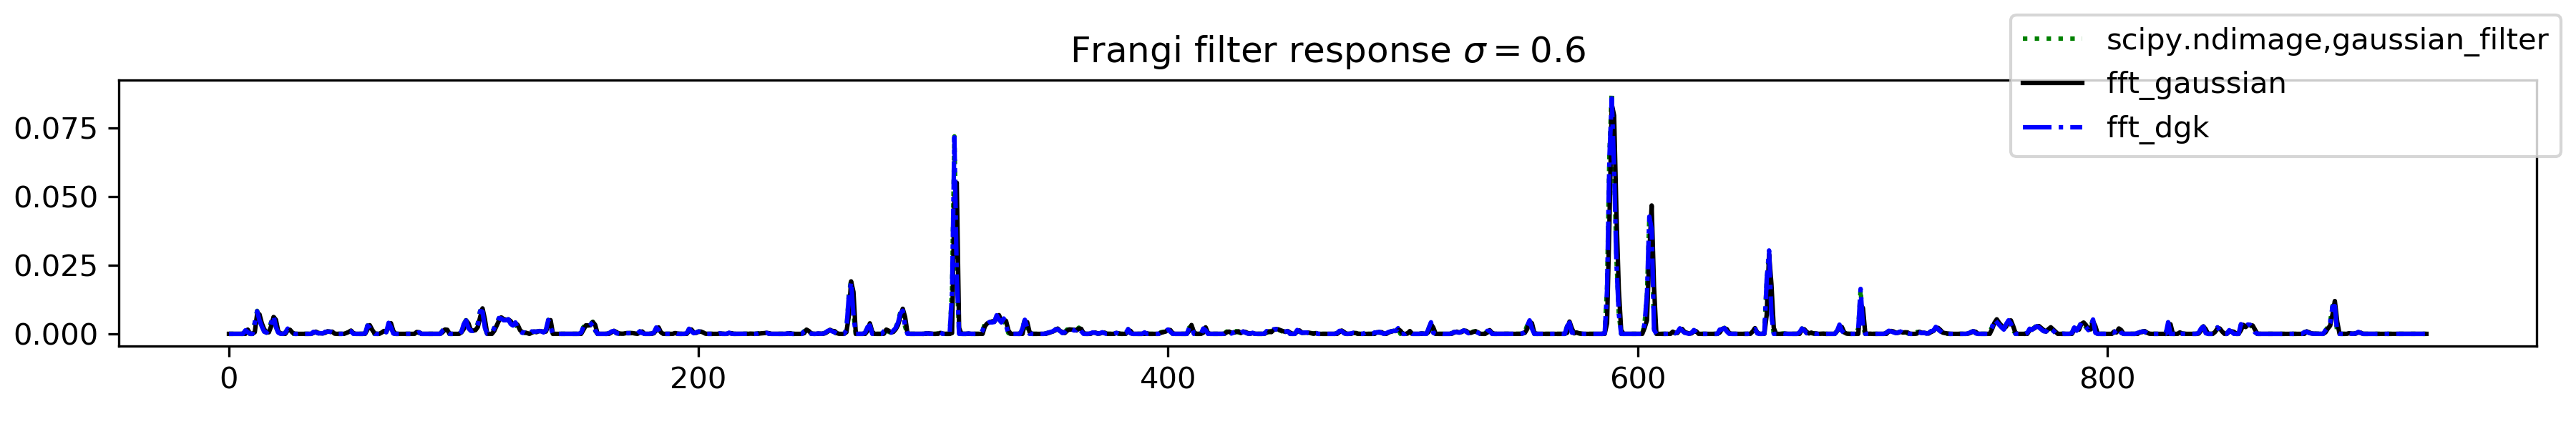
\includegraphics[width=\linewidth]{Fslice_sigma=6}
  \caption{Image cross-section of Gaussian blurred images $\sigma=5$}
  \label{fig:cross-sec-G-sigma=5}
\end{figure}

\begin{figure}
  \centering
  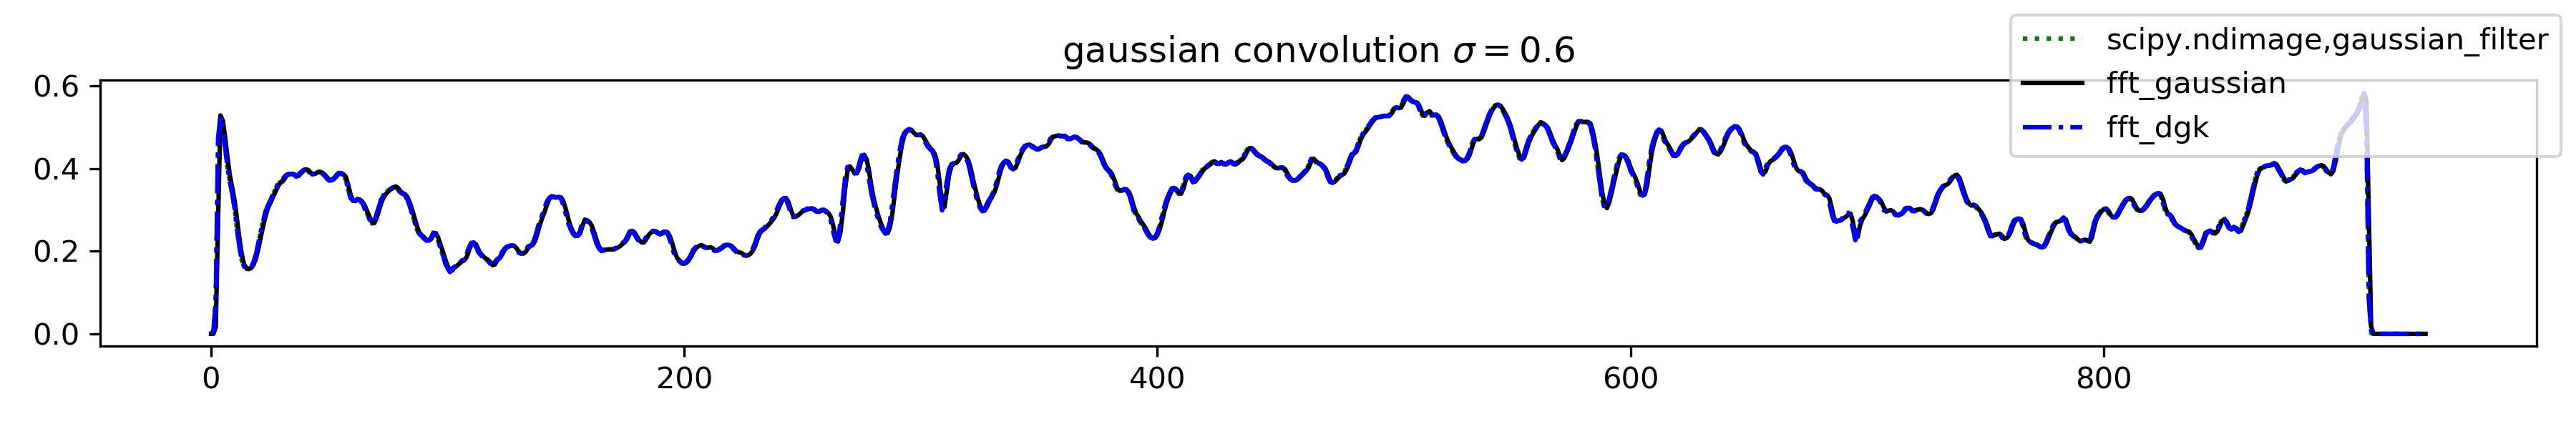
\includegraphics[width=\linewidth]{Gslice_sigma=6}
  \caption{Image cross-section of Frangi targets images $\sigma=5$}
  \label{fig:cross-sec-F-sigma=5}
\end{figure}


Finally, we wish to demonstrate the point of this comparison--that $FFT-based$ convolution is much faster than spatial convolution. We took a much larger sample ( 2200 by 2561) and timed each method of convolution (average of three trials) for a large number of samples: logarithmic between $\sigma=1$ and $\sigma=128$ with 32 steps. The result shows that the convolution time seems to at least linearly increase with the size of the kernel, whereas fft convolution behaves independently.

Frangi filtering

\begin{figure}
  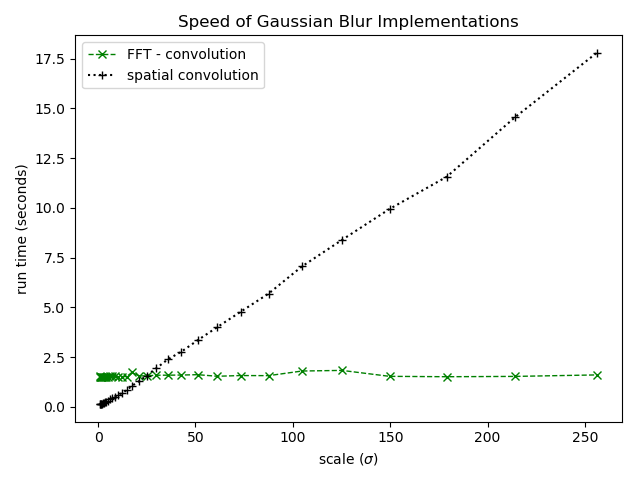
\includegraphics[width=\linewidth]{convolution-runtime-demo}
  \caption{Time required}
\end{figure}